\documentclass[12pt,letterpaper]{article}
\usepackage{fullpage}
\usepackage[top=2cm, bottom=4.5cm, left=2.5cm, right=2.5cm]{geometry}
\usepackage{amsmath,amsthm,amsfonts,amssymb,amscd}
\usepackage{lastpage}
\usepackage{enumitem}
\usepackage{fancyhdr}
\usepackage{mathrsfs}
\usepackage{xcolor}
\usepackage{graphicx}
\usepackage{listings}
\usepackage{hyperref}
\usepackage{palatino}
\usepackage{natbib}
\usepackage{xcolor}
\usepackage[capitalize]{cleveref}
\usepackage{xspace}
\usepackage{inconsolata}
\usepackage{tikz}

\newcommand{\transpose}{\mathsf{T}}
\newcommand{\hadamard}{\odot}

\definecolor{param_color}{rgb}{0.82352941, 0.91764706, 0.96862745}
\definecolor{data_color}{rgb}{0.96078431, 0.8627451 , 0.85490196}
\definecolor{param_color_dark}{rgb}{0.2, 0.6, 1.0}
\definecolor{data_color_dark}{rgb}{1.0, 0.4, 0.38}
\definecolor{comp_graph_param_grad_bcolor}{rgb}{0.97,0.88,0.35}

% https://tex.stackexchange.com/questions/27279/how-to-make-an-arrow-bigger-and-change-its-color-in-tikz/27287#27287
\tikzset{
  nn_edge/.style={
    decoration={markings,mark=at position 1 with {\arrow[scale=0.9]{spaced latex}}},
    postaction={decorate},
    shorten >=3.0pt
}}

\usetikzlibrary{arrows,arrows.spaced,arrows.meta,decorations.markings,calc,plotmarks}

\input{math_notation}
\newcommand{\given}{\mathrel{\vert}}
\newcommand*{\eg}{e.g.\@\xspace}
\newcommand*{\ie}{i.e.\@\xspace}
\newcommand*{\Eg}{E.g.\@\xspace}
\newcommand*{\Ie}{I.e.\@\xspace}
\newcommand*{\esp}{esp.\@\xspace}
\newcommand*{\wrt}{\ifmmode \stext{w.r.t.} \else w.r.t.\@\xspace \fi}
\newcommand*{\aever}{\ifmmode \stext{a.e.} \else a.e.\@\xspace \fi}
\newcommand*{\asurely}{\ifmmode \stext{a.s.} \else a.s.\@\xspace \fi}
% \newcommand*{\st}{\ifmmode \stext{s.t.} \else s.t.\@\xspace \fi}
\newcommand*{\wprob}{\ifmmode \stext{w.p.} \else w.p.\@\xspace \fi}
\newcommand*{\etc}{%
    \@ifnextchar{.}%
        {etc}%
        {etc.\@\xspace}%
}
\newcommand{\lhs}[0]{\hspace{2em}&\hspace{-2em}}
\newcommand{\trieq}[0]{\triangleq}
\newcommand{\eqin}[1]{\overset{#1}{=}}
\newcommand{\defeq}[0]{\overset{\mbox{\normalfont\tiny def}}{=}}

\hypersetup{%
  colorlinks=true,
  linkcolor=blue,
  linkbordercolor={0 0 1},
  citecolor=[rgb]{0,0.55,0.27}
}
 
\renewcommand\lstlistingname{Algorithm}
\renewcommand\lstlistlistingname{Algorithms}
\def\lstlistingautorefname{Alg.}

\lstdefinestyle{Python}{
    language        = Python,
    frame           = lines, 
    basicstyle      = \footnotesize,
    keywordstyle    = \color{blue},
    stringstyle     = \color{green},
    commentstyle    = \color{red}\ttfamily
}

\setlength{\parindent}{0.0in}
\setlength{\parskip}{0.1in}
\setlist[enumerate]{parsep=5pt}

% Edit these as appropriate
\newcommand\course{6.S898 Deep Learning}
\newcommand\hwnumber{1}                  % <-- homework number

\pagestyle{fancyplain}
\headheight 40pt
\lhead{}
% \lhead{\NetIDa}
% \lhead{\NetIDa\\\NetIDb}                 % <-- Comment this line out for problem sets (make sure you are person #1)
\chead{\textbf{\Large Math Notation}}
\rhead{\course \\ Fall 2023}
\lfoot{}
\cfoot{}
\rfoot{\small\thepage}
\headsep 1.5em

\newcommand{\fixme}[1]{{\color{red} \bf FIXME: #1}}
\newcommand{\answer}[1]{{\color{red}\textbf{Answer}: #1}}
% \renewcommand{\answer}[1]{}

\begin{document}

\newcommand{\xin}{\mathbf{x}_{\texttt{in}}}
\newcommand{\xout}{\mathbf{x}_{\texttt{out}}}
\newcommand{\xini}{x_{\texttt{in}_i}}
\newcommand{\xouti}{x_{\texttt{out}_i}}
\newcommand{\xink}{x_{\texttt{in}_k}}

In deep learning we encounter many different fields and each has its own notation. We will stick to the following conventions throughout most of this course, and note it when we deviate from these rules. To define the conventions we give examples of usage, from which you can infer the pattern.

\paragraph{General notation}
\begin{itemize}
\item Scalar: $x$, $y$, $z$.
\item Vector: $\mathbf{x}, \mathbf{y}, \mathbf{z}$. We use bold letters to represent vectors, matrices, and tensors.
\item Index of a vector: $x_i$, $x_j$, $y_i$, or $x[i]$, $x[j]$, $y[i]$.
\item Matrix: $\mathbf{X}$, $\mathbf{Y}$, $\mathbf{Z}$. We use bold letters to represent vectors, matrices, and tensors.
\item Index of a matrix: $X_{ij}$, $Y_{jk}$, $Z_{ii}$, or $X[i,j]$, $Y[j,k]$, $Z[i,i]$.
\item For an indexed matrix $X_{ij}$ or $X[i,j]$, $i$ indexes rows and $j$ indexes columns. We use non bold font because $X_{ij}$ and $X[i,j]$ are scalars.
\item Slice of a matrix: $\mathbf{X}_i$ or $\mathbf{X}[i,:]$; $\mathbf{X}[:,j]$. Here is one example:
\begin{align*}
\mathbf{X} = 
\begin{bmatrix}
    1 & 2 \\
    3 & 4 \\
    5 & 6
\end{bmatrix}
&&
\mathbf{X}[2,:] = 
\begin{bmatrix}
    3 & 4
\end{bmatrix}
\end{align*}
\item Tensor (i.e., multidimensinoal arrays): Typically, we will use lowercase bold variables to represent tensors, for example, $\mathbf{x}$. This is because tensors can have any number of dimensions (they can be one-dimensional, two-dimensional, three-dimensional, and so on). Furthermore, we will often define operators that are agnostic to the dimensionality of the tensor (they apply to $N$-dimensional arrays, for any $N$). However, in some sections, we use uppercase to make a distinction between tensors of different shapes, and we will specify when this is the case. 
\item Index or slice of a tensor: $x[c,i,j,k]$, $\mathbf{x}[:,:,k]$
%\item When the dimensionality of a variable is arbitrary (can take on different values in different settings) we will consider it a tensor and use the tensor notation.
\item A set of $N$ datapoints: $\{x^{(i)}\}_{i=1}^N$, $\{\mathbf{x}^{(i)}\}_{i=1}^N$, $\{\mathbf{X}^{(i)}\}_{i=1}^N$
%\item $\mathbf{A} = [\mathbf{x},\mathbf{y},\mathbf{z}]$ concatenates column vectors $\mathbf{x},\mathbf{y},\mathbf{z}$ as columns of matrix $A$. $\mathbf{A} = [\mathbf{x}^\transpose,\mathbf{y}^\transpose,\mathbf{z}^\transpose]$ concatenates these vectors as rows of $\mathbf{A}$. 
\item Dot product: $\mathbf{x}^\transpose\mathbf{y}$
\item Matrix product: $\mathbf{A}\mathbf{B}$
\item Hadamard product (i.e., element-wise product): $\mathbf{x} \hadamard \mathbf{y}$, $\mathbf{A} \hadamard \mathbf{B}$
\item Product of two scalars: $ab$ or $a*b$ 
\end{itemize}

\paragraph{Machine learning}
\begin{itemize}
    \item Loss function: $\mathcal{L}$ (usually this is a per-datapoint loss)
    \item Total cost over all datapoints: $J$
    \item Generic learnable parameters: $\theta$
\end{itemize}


\paragraph{Neural nets}
\begin{itemize}
\item \textit{Parameters}: $\theta$; these include weights, $\mathbf{W}$, and biases, $\mathbf{b}$, as well as any other learnable parameters of a network.
\item \textit{Data}: $\mathbf{x}$ -- ``Data" can refer to inputs to the network, activations on hidden layers, outputs from the network, etc. Any representation of the signal being processed is considered to be ``data". Sometimes we will wish to distinguish between the raw inputs, hidden units, and outputs to a network, in which case we will use $\mathbf{x}$, $\mathbf{h}$, and $\mathbf{y}$ respectively. When we need to to distinguish between pre-activation hidden units and post-activation, we will use $\mathbf{z}$ for pre-activation and $\mathbf{h}$ for post-activation.

\item When describing batches of tensors (as is commonly encountered in code), you may encounter $x_l[b,c,n,m]$ to represent an activation on layer $l$ of some network, with $b$ indexing batch element, $n$ and $m$ as spatial coordinates, and $c$ indexing channels.
\item Neuron values on layer $l$ of a deep net: $\mathbf{x}_{l}$
\item $x_{l}[n]$ refers to the $n$-th neuron on layer $l$. For neural networks with spatial feature maps (such as convolutional neural networks), each layer is an array of neurons, and we will use notation such as $x_{l}[n,m]$ to index the neuron at location $n,m$.
%\item For a network with spatial feature maps (e.g., a convolutional neural network), $x_{l}[c,i,j]$ refers to the $cij$-th neuron on layer $l$, where $i$ and $j$ index spatial position in a feature map, and $c$ indexes the channel.
\item The layer $l$ neural representation of the $i$-th datapoint in a dataset is written as $\mathbf{x}^{(i)}_{l}$.
\item We will also use $\xin$ and $\xout$ when we are describing a particular layer or module in a neural net and wish to speak of its inputs and outputs without having to keep track of layer indices.
\item For signals with multiple channels, including neural network feature maps, the first dimension of the tensor indexes over channel. For example, in $\mathbf{x} \in \mathbb{R}^{C \times N \times M \times \ldots}$, where $C$ is the number of channels of the signal.
\item For transformers, we deviate from the previous point slightly, in order to match standard notation: a set of tokens (which will be defined in the transformers chapter) is represented by a $[N \times d]$ matrix, where $d$ is the token dimensionality.
\end{itemize}


We will use circles to represents neurons, which are scalar nodes in a graph. Edges between neurons represent a $\mathbb{R} \rightarrow \mathbb{R}$ transformation (usually parameterized by a single weight associated with the edge). In many neural net architectures, the nodes of our networks are not individual neurons, but instead may be multidimensional vectors of neurons, which we will draw as squares or rectangles. In these cases, an edge between a node of dimensionality $C_1$ and a node of dimensionality $C_2$ represents a $\mathbb{R}^{C_1} \rightarrow \mathbb{R}^{C_2}$ transformation (which may be parameterized by multiple weights). The three node symbols we use are shown below:
\begin{figure}[h!]
    \def\layerheight{1.2}
    \def\neuronrad{0.15}
    \begin{minipage}{0.32\linewidth}
    \centering
    \begin{tikzpicture}
        \begin{scope}[rotate=-90]
        \draw [fill=white] (0,0) circle (\neuronrad);
        \draw [thin] [nn_edge] (0,\neuronrad) -- (0,\layerheight-\neuronrad);
        \draw [fill=white] (0,\layerheight) circle (\neuronrad);
        %
        \draw (-\neuronrad*3.5,0) node {\small scalar};
        \draw (-\neuronrad*3.5,\layerheight) node {\small scalar};
        \end{scope}
    \end{tikzpicture}
    \end{minipage}
    \begin{minipage}{0.32\linewidth}
    \centering
    \begin{tikzpicture}
        \begin{scope}[rotate=-90]
        \draw [fill=white] (-\neuronrad,-\neuronrad) rectangle ++(\neuronrad*2,\neuronrad*2);
        \draw [thin] [nn_edge] (0,\neuronrad) -- (0,\layerheight-\neuronrad);
        \draw [fill=white] (-\neuronrad,-\neuronrad+\layerheight) rectangle ++(\neuronrad*2,\neuronrad*2);
        %
        \draw (-\neuronrad*3.5,0) node {\small vector};
        \draw (-\neuronrad*3.5,\layerheight) node {\small vector};
        \end{scope}
    \end{tikzpicture}
    \end{minipage}
    \begin{minipage}{0.32\linewidth}
    \centering
    \begin{tikzpicture}
        \draw [fill=white] (-\neuronrad/2,-\neuronrad*2) rectangle ++(\neuronrad,\neuronrad*4);
        \draw [thin] [nn_edge] (0,\neuronrad*2) -- (0,\layerheight-\neuronrad*2);
        \draw [fill=white] (-\neuronrad/2,-\neuronrad*2+\layerheight) rectangle ++(\neuronrad,\neuronrad*4);
        %
        \draw (\neuronrad*9.25,0) node {\small vector (token)};
        \draw (\neuronrad*9.25,\layerheight) node {\small vector (token)};
    \end{tikzpicture}
    \end{minipage}
    %\caption{Notation conventions for neural network nodes.}
    %\label{fig:convolutional_neural_nets:network_node_notation}
\end{figure}

A token is a vector of neurons used in a particular way, which will be defined in the transformers chapter. We give it a special symbol, a rectangle, to distinguish it from other kinds of vectors of neurons.

As shown above, sometimes we draw networks with the layers moving left to right and sometimes bottom to top. Both mean the same thing, and the direction in each figure is just chosen for visual clarity.



\paragraph{Probabilities}\mbox{}\\
We will typically not distinguish between random variables and realizations of those variables; which we mean should be clear from context. When it is important to make a distinction, we will use non-bold capital letters to refer to random variables and lowercase to refer to realizations.

Suppose $X, Y$ are discrete random variables and $\mathbf{x}, \mathbf{y}$ are realizations of those variables. $X$ and $Y$ may take on values in the sets $\mathcal{X}$ and $\mathcal{Y}$ respectively.
\begin{itemize}
    \item $a = p(X = \mathbf{x} | \ldots)$ is the probability of the realization $X = \mathbf{x}$, possibly conditioned on some observations ($a$ is a scalar).
    \item $f = p(X | \ldots)$ is the probability distribution over $X$, possibly conditioned on some observations ($f$ is a function: $f: \mathcal{X} \rightarrow \mathbb{R}$). If $\mathcal{X}$ is discrete, $f$ is the \emph{probability mass function}. If $\mathcal{X}$ is continuous, $f$ is the \emph{probability density function}.
    %\item $a = p(X = x | \overset{R}{y} = y)$ is the probability of the realization $\overset{R}{x}=x$ given $\overset{R}{y}=y$ ($a$ is a scalar).
    %\item $f = p(\overset{R}{x} | \overset{R}{y} = y)$ is the probability distribution over $\overset{R}{x}$ given $\overset{R}{y}=y$ ($f: \mathcal{X} \rightarrow \mathbb{R}$).
    %\item $f = p(\overset{R}{x} = x | \overset{R}{y})$ is a function with the property $f(y) = p(\overset{R}{x} = x | \overset{R}{y} = y)$ ($f: \mathcal{Y} \rightarrow \mathbb{R}$).
    %\item $p(\overset{R}{x} | \overset{R}{y})$ is the conditional probability distribution of $\overset{R}{x}$ given $\overset{R}{y}$ ($f: \mathcal{X} \times \mathcal{Y} \rightarrow \mathbb{R}$).
    %\item $p(x)$ is shorthand for $p(\overset{R}{x} = x)$.
    %\item $p(x|y)$ is shorthand for $p(\overset{R}{x} = x | \overset{R}{y} = y)$.
    %\item Suppose we have defined a named distribution, e.g., $p_{\theta}$; then referring to $p_{\theta}$ on its own is shorthand for $p(\overset{R}{x})$. This often comes up in expressions like $x \sim p_{\theta}$, which refers to $\overset{R}{x}$ as being distributed as $p_{\theta}(\overset{R}{x})$.
    %\item $p(\overset{R}{x} | y)$ is shorthand for $p(\overset{R}{x} | \overset{R}{y} = y)$
    \item $p(\mathbf{x} | \ldots)$ is shorthand for $p(X = \mathbf{x} | \ldots)$.
    %\item $p(\ldots | y)$ is shorthand for $p(\ldots | \overset{R}{y} = y)$.
    \item and so forth, following these patterns.
    \item Suppose we have defined a named distribution, e.g., $p_{\theta}$; then referring to $p_{\theta}$ on its own is shorthand for $p_{\theta}(X)$
\end{itemize}
For continuous random variables, all the above notations hold except that they refer to probability densities and probability density functions rather than probabilities and probability distributions. We will sometimes use the term ``probability distribution" when referring to continuous distributions, and in those cases this should be understood to refer to a probability density function.

\paragraph{Matrix calculus conventions}

In these notes, we adopt the following conventions for matrix calculus. These conventions make the equations simpler, and that also means simpler implementations when it comes to actually writing these equations in code. Everything in this section is just definitions. There is no right or wrong to it. We could have used other conventions but we will see that these are useful ones.

Vectors are represented as column vectors with shape $[N \times 1]$:
\begin{align}
    \mathbf{x} \triangleq 
    \begin{bmatrix}
    x_1  \\
    x_2  \\
    \vdots \\
    x_N \\
    \end{bmatrix}
\end{align}
If $y$ is a scalar and $\mathbf{x}$ is an $N$-dimensional vector, then the gradient $\frac{\partial y}{\partial \mathbf{x}}$ is a row vector of shape  $[1 \times N]$:
\begin{align}
    \frac{\partial y}{\partial \mathbf{x}} \triangleq  
\begin{bmatrix}
    \frac{\partial y}{\partial x_1} & \frac{\partial y}{\partial x_2} & \cdots & \frac{\partial y}{\partial x_N} \label{backprop:scalar_vector_deriv}
\end{bmatrix}
\end{align}
If $\mathbf{y}$ is an $M$-dimensional vector and $\mathbf{x}$ is a $N$-dimensional vector then the gradient (also called the Jacobian in this case) is shaped as $[M \times N]$:
\begin{align}
\frac{\partial \mathbf{y}}{\partial \mathbf{x}} \triangleq  
\begin{bmatrix}
    \frac{\partial y_1}{\partial x_1} & \frac{\partial y_1}{\partial x_2} & \cdots & \frac{\partial y_1}{\partial x_N} \\
    \vdots & \vdots & \vdots & \vdots \\
    \frac{\partial y_M}{\partial x_1} & \frac{\partial y_M}{\partial x_2} & \cdots & \frac{\partial y_M}{\partial x_N}
\end{bmatrix}
\end{align}


Finally, if $\mathbf{W}$ is an $[N \times M]$ dimensional matrix, and $\mathcal{L}$ is a scalar, then the gradient $\frac{\partial \mathcal{L}}{\mathbf{W}}$ is represented as an $[M \times N]$ dimensional matrix (note that the dimensions are transposed from what you might have expected; this makes the math simpler later):
\begin{align}
    \frac{\partial \mathcal{L}}{\partial \mathbf{W}} &\triangleq 
        \begin{bmatrix}
            \frac{\partial \mathcal{L}}{\partial \mathbf{W}_{11}} & \ldots & \frac{\partial \mathcal{L}}{\partial \mathbf{W}_{N1}} \\
            \vdots & \ddots & \vdots \\
            \frac{\partial \mathcal{L}}{\partial \mathbf{W}_{1M}} & \ldots & \frac{\partial \mathcal{L}}{\partial \mathbf{W}_{NM}} \\
        \end{bmatrix} \label{backprop:scalar_matrix_deriv}
\end{align}

\newpage
We will sometimes draw matrices and vectors to help visualize the operations. For example, if $N=3$ and $M=4$:\\
\begin{figure}[h!]
\centerline{
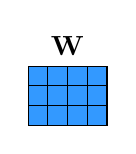
\begin{tikzpicture}
\draw[step=0.25cm,draw=black,fill=param_color_dark] (1.5,0) grid (2.5,-0.75) rectangle (1.5,0); \node at (2.0,0.25) {$\mathbf{W}$};
\end{tikzpicture}}
\end{figure}

then, the gradient will have the form:\\
\begin{figure}[h!]
\centerline{
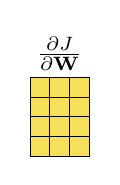
\begin{tikzpicture}
\draw[step=0.25cm,draw=black,fill=comp_graph_param_grad_bcolor] (0,0) grid (0.75,-1.0) rectangle (0,0); \node at (0.375,0.3) {$\frac{\partial J}{\partial \mathbf{W}}$};
\end{tikzpicture}}
\end{figure}

\paragraph{Conventions that will not be strictly adhered to}
\begin{itemize}
\item We will often use $\mathbf{x}$ as the input to a function, and $\mathbf{y}$ as the output.
\item $f$, $g$, and $h$ are typically functions. The corresponding function spaces are $\mathcal{F}$, $\mathcal{G}$, $\mathcal{H}$.
\end{itemize}

\paragraph{Miscellaneous}
\begin{itemize}
\item The word {\bf dimension} has two usages in the computational sciences. The first usage is as a coordinate in a multivariate data structure, for example, ``the $i$-th dimension of a vector'' or ``a 128-dimensional feature space.'' The second usage is as the shape of a multidimensional array, as in ``a 4D tensor.'' We will use both these meanings in this book and we hope the usage will be clear from context.
\end{itemize}

\end{document}